\def\topic{Dynamically defined Schr\"odinger kernels}
\ifdefined\MyHeaderIncluded
\else
\def\qwertyflag{true}

\ifdefined\MyHeaderIncluded

\else
  \newcommand{\foobar}{FooBar}
  \def\MyHeaderIncluded{true}
% if is till the end of the file

\documentclass[10pt,a4paper]{article}
\usepackage[utf8]{inputenc}
%\usepackage[german]{babel}
%\usepackage[cyrillic]{babel}
\usepackage[T1]{fontenc}
%\usepackage[T2A]{fontenc}
%\usepackage[english, russian]{babel}
\usepackage{amsmath}
\usepackage{amsfonts}
\usepackage{amssymb}
\usepackage{amsthm}
\usepackage{mathtools} %coloneqq

\usepackage{bussproofs} %

%\renewcommand{\thesubsection}{\arabic{subsection}}
%\newtheorem{thm}{Theorem}[section]
%\renewcommand{\thethm}{\arabic{subsection}.\arabic{thm}}

\usepackage{thmtools}
\usepackage{hyperref}
\hypersetup{
    colorlinks=true,
    linkcolor=blue,
    filecolor=magenta,      
    urlcolor=cyan,
    pdftitle={Overleaf Example},
    %pdfpagemode=FullScreen,
    }
%\usepackage{stix-type1}%\turnediota
\theoremstyle{definition}

\newtheorem{constructor}{Constructor}[section]
\newtheorem{iaxiom}{Axiom}
\newtheorem{axiom}{Axiom}
\newtheorem*{axiom*}{Axiom}
\newtheorem{definition}{Definition}[section]
\newtheorem*{definition*}{Definition}
\newtheorem{remark}{Remark}[section]
\newtheorem*{remark*}{Remark}
\newtheorem{recall}{Recall}[section]
\newtheorem*{recall*}{Recall}

\newtheorem{lemma}{Lemma}[section]
\newtheorem{theorem}{Theorem}[section]
\newtheorem*{theorem*}{Theorem}
\newtheorem{note}{Note}[section]
\usepackage{etoolbox}

%\newcommand*{\@Dashv}[2]{%
%  \reflectbox{$\m@th#1#2$}%
%}
\newcommand*{\separation}[3]{% 1)binder, 2)set, 3)condition
  \{#1\in #2: #3\}
}

% https://www.freecodecamp.org/news/simple-regex-tricks-for-beginners-3acb3fa257cb/
%  \\mathcal\{T\} |---> \topology
%  \\mathcal\{([^\}]*)\}   |--->  $1
\newcommand{\AND}{\ \ \&\ \ }
\newcommand{\any}{\mathrm{\ any}}
\newcommand{\borel}{\mathcal{B}}
\newcommand{\can}{\mathrm{can}}
\newcommand{\canonize}{\mathrm{canonize}}
\newcommand{\closure}{\mbox{cl}}
\newcommand{\complex}{\mathbb{C}}
\newcommand{\converges}{\longrightarrow}
\newcommand{\countable}{\mbox{\ countable}}
\newcommand{\ldefined}{\mbox{\ defined}}
\newcommand{\dom}{\mbox{dom}}
\newcommand{\Dom}{\mbox{Dom}}
\newcommand{\Done}{\noindent \textbf{Done.}\\}
\newcommand{\lexists}{\mbox{\ exists}}
\newcommand{\lforall}{\mbox{\ forall}}
\newcommand{\lunique}{\mbox{\ unique}}
\newcommand{\family}{\mathrm{\ family}}
\newcommand{\Fm}{\mathrm{Fm}}
\newcommand{\FuncSymb}{\mathrm{FuncSymb}}
\newcommand{\function}{\mathrm{\ function}}
\newcommand{\functional}{\mbox{\ functional}}
\newcommand{\IFF}{\ \Longleftrightarrow\ }
\renewcommand{\iff}{\ \longleftrightarrow\ }
\newcommand{\IMPLIES}{\ \Longrightarrow\ }
\renewcommand{\implies}{\ \longrightarrow\ }
\newcommand{\Inf}{\mathrm{Inf}}
\newcommand{\injective}{\mbox{\ injective}}
\newcommand{\injection}{\mbox{\ injection}}
\newcommand{\interior}{\mbox{int}}
\newcommand{\intersection}{\bigcap}
\newcommand{\isempty}{\mathrm{\ empty}}
\newcommand{\LB}{\mathrm{LB}}
\newcommand{\nghbset}{\mathcal{N}}
\newcommand{\nonempty}{\mathrm{\ nonempty}}
\newcommand{\Ord}{\mathrm{Ord}}
\newcommand{\power}{\mathcal{P}}
\newcommand{\pr}{\mathrm{pr}}
\newcommand{\fst}{\mathrm{fst}}
\newcommand{\snd}{\mathrm{snd}}
\newcommand{\PredSymb}{\mathrm{PredSymb}}
\newcommand{\Proof}{\noindent \textbf{Proof.}\\}
\newcommand{\ran}{\mathrm{ran}}
\newcommand{\Ran}{\mathrm{Ran}}
\newcommand{\real}{\mathbb{R}}
\newcommand{\relation}{\mathrm{\ relation}}
\newcommand{\set}{\mathrm{\ set}}
\newcommand{\singleton}{\mathrm{\ singleton}}
\newcommand{\semantics}{\mathrm{semantics}}
\newcommand{\semialgebra}{\mathcal{S}}
\newcommand{\Sup}{\mathrm{Sup}}
\newcommand{\surjective}{\mbox{\ surjective\ on\ }}
\newcommand{\Term}{\mathrm{Term}}
\newcommand{\Type}{\mathrm{Type}}
\newcommand{\topology}{\mathcal{T}}
\newcommand{\total}{\mbox{\ total\ on\ }}
\newcommand{\transitive}{\mathrm{\ transitive}}
\newcommand{\union}{\bigcup}
\newcommand{\lTrue}{\mathrm{True}}
\newcommand{\lFalse}{\mathrm{False}}
\newcommand{\lUncertain}{\mathrm{Uncertain}}
\newcommand{\lif}{\mathrm{if}}
\newcommand{\lthen}{\mathrm{then}}
\newcommand{\lelse}{\mathrm{else}}
\newcommand{\lexception}{\mathrm{exception}}
\newcommand{\lundef}{\mathrm{undef}}
\newcommand{\univocal}{\mathrm{\ univocal}}
\newcommand{\univocalat}{\mathrm{\ univocal\ at\ }}
\newcommand{\UB}{\mathrm{UB}}
\newcommand{\Un}{\mathcal{U}}
\newcommand{\Var}{\mathrm{Var}}

\newcommand{\notvarphi}{\phi}
\renewcommand{\phi}{\varphi}

\newcommand{\comment}[1]{\quad\mbox{(#1)}}
% local commands
%\preto\section{\undef\blipo} %etoolbox
\preto\subsection{\undef\blipo} %etoolbox
% https://tex.stackexchange.com/questions/105684/limit-macro-newcommand-scope-to-section
\usepackage{graphicx}
\usepackage{authblk}

\setlength\parindent{0pt} % whole doc of \noindent
\usepackage{soul}
%\usepackage{mathgl}

\fi % guard
\ifdefined\topic
\else
\def\topic{No Titel}
\fi
\title{\topic}
\author[1]{Georgy Dunaev}
\begin{document}
\maketitle
\fi
\section{Dynamically defined Schr\"odinger kernels}
\label{sec:dynamical_schrodinger}
We address the parameter-regularity question for a compact dynamical
system. The argument gives a quantitative Lipschitz estimate under the
stated linear growth bound for the action. It is a proof under these
hypotheses, not a claim that the result is new in the literature.

The baseline quantitative results use Lipschitz sampling and the linear
action bound~\eqref{eq:dynamic_action_bound}; isometric actions give
sharper constants. The H\"older extension retains that action bound
and weakens only the sampling assumption, whereas the exponential-action
extension retains Lipschitz sampling and replaces the action bound.
These extensions are stated separately. The localized operator-norm
Lipschitz estimate uses the baseline assumptions. Finally,
Proposition~\ref{prop:dynamic_strong_parameter_continuity} requires only
continuous sampling and a continuous action on a compact metric space,
with no quantitative action bound. The final quantitative subsystem spectral estimates
return to the baseline Lipschitz and linear-growth assumptions; their
qualitative counterpart requires only continuity.

\subsection{The hypotheses and translation convention}
Let $(Z,d_Z)$ be a nonempty compact metric space, and let
$T:\mathbb R^d\times Z\to Z$ be a continuous action:
\[
T(0,z)=z,\qquad T(g,T(h,z))=T(g+h,z).
\]
Assume that a constant $C\geq0$ satisfies
\[
d_Z(T(g,z),T(g,w))\leq C(1+|g|)d_Z(z,w).
\tag{D}\label{eq:dynamic_action_bound}
\]
Let $v:Z\to\mathbb R$ have Lipschitz constant $L$, and put
$M=\|v\|_\infty=\sup_{z\in Z}|v(z)|<\infty$. Define
\[
V_z(g)=v(T(g,z)),\qquad H_z=H_0+V_z,\qquad
H_0=-\sum_{j=1}^d\partial_j^2.
\]
Each $V_z$ is continuous and bounded by $M$. Write
$K_z(t,g,h)=k_{V_z}(t,g,h)$ for its continuous kernel and set
\[
k_t(z,r)=K_z(t,0,r),\qquad t>0.
\]
The actual potential difference is bounded by $2M$ and also satisfies
\[
|V_z(u)-V_w(u)|\leq LC(1+|u|)d_Z(z,w).
\tag{P}\label{eq:dynamic_potential_difference}
\]
The latter bound grows in $u$; it will be integrated against a Gaussian,
not used as a uniform bound for a multiplication operator.

\begin{proposition}[Pointwise covariance]
\label{prop:dynamic_covariance}
For $t>0$ and $g,h\in\mathbb R^d$,
\[
K_z(t,g,h)=k_t(T(g,z),h-g).
\tag{C}\label{eq:dynamic_covariance}
\]
Consequently, for every $\psi\in L^2(\mathbb R^d)$,
\[
(e^{-tH_z}\psi)(g)
 =\int_{\mathbb R^d}k_t(T(g,z),h-g)\psi(h)\,dh,
\]
where the left side denotes the continuous representative constructed
in Theorem~\ref{thm:bounded_schrodinger_kernel}.
\end{proposition}
\Proof
The action law gives $V_{T(g,z)}(u)=V_z(u+g)$. Translation invariance
of the Gaussian and a change of variable in each Dyson integral give,
by induction on its order,
\[
k_n^{V_{T(g,z)}}(t,a,b)=k_n^{V_z}(t,a+g,b+g).
\]
Summing the absolutely convergent series and taking $a=0$, $b=h-g$
proves the pointwise identity. The integral against $\psi$ converges
absolutely by the Gaussian bound and Cauchy--Schwarz; the kernel theorem
identifies it with the stated continuous representative.
\Done

The sign is fixed by the potential convention. If instead
$\widetilde V_z(g)=v(T(-g,z))$, the same proof gives
\[
(e^{-t\widetilde H_z}\psi)(g)
 =\int_{\mathbb R^d}\widetilde k_t(T(-g,z),h-g)\psi(h)\,dh.
\]
Thus a covariant kernel formula containing $T(-g,z)$ corresponds to
the negative-action potential convention. Keeping $V_z(g)=v(T(g,z))$ requires the plus sign.
All estimates below hold in either convention, since the action bound
also applies to $-g$.

\subsection{A pointwise Duhamel comparison}
We temporarily return to arbitrary bounded real potentials. The
comparison identity below is independent of the dynamical assumptions;
applying it to $V_z$ and $V_w$ will provide the parameter estimates.
\begin{lemma}[Comparison of continuous kernel representatives]
\label{lem:kernel_duhamel_comparison}
Let $V,W$ be real bounded measurable potentials with norms at most $M$.
At every $t>0$ and every $x,y\in\mathbb R^d$,
\[
\begin{split}
k_V(t,x,y)-k_W(t,x,y)
=-\int_0^t\int_{\mathbb R^d}
 &k_V(t-s,x,u)[V(u)-W(u)]\\[-2pt]
 &\hspace{12mm}\cdot k_W(s,u,y)\,du\,ds.
\end{split}
\tag{DK}\label{eq:kernel_duhamel_comparison}
\]
The integral is absolutely convergent and jointly continuous in $t,x,y$.
\end{lemma}
\Proof
The two operators have common domain $D(H_0)$. Differentiating
$e^{-(t-s)(H_0+V)}e^{-s(H_0+W)}f$ there, as in
Lemma~\ref{lem:schrodinger_duhamel}, and then extending by density gives
\[
e^{-t(H_0+V)}-e^{-t(H_0+W)}
=-\int_0^t e^{-(t-s)(H_0+V)}(V-W)e^{-s(H_0+W)}\,ds.
\]
This is initially a strong operator identity. Gaussian convolution
bounds the absolute spatial integral of its proposed kernel by
$e^{Mt}\|V-W\|_\infty p_t(x-y)$, independently of $s$.
The double integral is therefore absolutely convergent and bounded by
$t e^{Mt}\|V-W\|_\infty p_t(x-y)$.

We check continuity before evaluating at a particular point such as
$x=0$. Put $s=t\theta$ and first retain
$\varepsilon\leq\theta\leq1-\varepsilon$. On compact parameter sets
with $t$ bounded away from zero, both kernels are continuous and the
integrand has an integrable Gaussian envelope in $u$. Dominated
convergence gives continuity of the truncated integral. The omitted
intervals contribute at most
\[
2\varepsilon t e^{Mt}\|V-W\|_\infty p_t(x-y),
\]
uniformly on these compact sets. The full integral is continuous.
Fubini against bounded compactly supported test functions identifies
its operator with the strong Duhamel integral. Continuous-kernel
uniqueness now proves the formula everywhere, not just almost everywhere.
\Done

\begin{corollary}[Potential order and scalar shifts]
\label{cor:kernel_potential_order}
Let $V,W$ be real bounded measurable potentials. If $V\leq W$
almost everywhere, then, for every $t>0$ and $x,y\in\mathbb R^d$,
\[
k_V(t,x,y)\geq k_W(t,x,y).
\]
Consequently, if real constants $m,b$ satisfy $m\leq V\leq b$
almost everywhere, then
\[
e^{-bt}p_t(x-y)\leq k_V(t,x,y)\leq e^{-mt}p_t(x-y).
\]
For every real constant $c$, one also has
\[
k_{V+c}(t,x,y)=e^{-ct}k_V(t,x,y).
\]
\end{corollary}
\Proof
Choose a common bound for the norms of $V,W$ and apply
Lemma~\ref{lem:kernel_duhamel_comparison}. Both kernel factors in
its integrand are nonnegative by
Proposition~\ref{prop:schrodinger_kernel_identities}. Since
$V-W\leq0$ almost everywhere, the leading minus sign makes their
integral nonnegative. This proves the comparison at every $x,y$.
Comparison with the constant potentials $b$ and $m$, whose kernels
are $e^{-bt}p_t$ and $e^{-mt}p_t$, gives the two-sided estimate.
Finally, scalar spectral translation gives
\[
e^{-t(H_0+V+c)}=e^{-ct}e^{-t(H_0+V)}.
\]
Both sides have continuous kernels, so continuous-kernel uniqueness
proves the shift identity pointwise.
\Done

The comparison also says that
$e^{-t(H_0+V)}f\geq e^{-t(H_0+W)}f$ for every nonnegative
$f\in L^2$, using the continuous representatives. This is order
on nonnegative functions; no inequality between quadratic forms of
these operators is asserted.

If a family of potentials has a common lower bound $m$, its kernels
are bounded above by $e^{-mt}p_t$. In a Duhamel comparison the two
kernel factors are therefore bounded by
\[
e^{-m(t-s)}p_{t-s}(x-u)\,e^{-ms}p_s(u-y)
=e^{-mt}p_{t-s}(x-u)p_s(u-y).
\]
Thus in the Duhamel-derived pointwise, weighted-norm, and localized
operator-norm parameter estimates below, the factor $e^{Mt}$ can be
replaced by $e^{-mt}$, including when it is combined with other
exponential factors. For the original dynamical family one may take
$m=\min_{z\in Z}v(z)$, which exists by continuity and compactness.
This improvement concerns these parameter comparison estimates; it
does not assert the same substitution in the separate spatial or
time derivative estimates.

\subsection{The Gaussian moment controlling parameter regularity}
\begin{lemma}[Weighted Gaussian convolution]
\label{lem:gaussian_bridge_moment}
For $0<s<t$ and $r\in\mathbb R^d$,
\[
\begin{split}
\int_{\mathbb R^d}(1+|u|)p_{t-s}(u)p_s(r-u)\,du
\leq p_t(r)\left(1+\frac{t-s}{t}|r|
                     +\sqrt{\frac{2d s(t-s)}{t}}\right).
\end{split}
\]
Consequently, with $c_d=\pi\sqrt{2d}/8$,
\[
\int_0^t\int_{\mathbb R^d}(1+|u|)p_{t-s}(u)p_s(r-u)\,du\,ds
\leq p_t(r)\left[t\left(1+\frac{|r|}{2}\right)+c_dt^{3/2}\right].
\]
\end{lemma}
\Proof
Completing the square gives
\[
p_{t-s}(u)p_s(r-u)=p_t(r)p_a(u-m),\qquad
a=\frac{s(t-s)}t,\quad m=\frac{t-s}t r.
\]
The density $p_a$ has mass one and second moment
$\int |q|^2p_a(q)\,dq=2da$, by one-dimensional Gaussian integration
in each coordinate. The triangle inequality and Cauchy--Schwarz give
\[
\int |u|p_a(u-m)\,du\leq |m|+\sqrt{2da}.
\]
This proves the first estimate. The mean term integrates to $t|r|/2$,
and the square-root term integrates to
\[
\sqrt{2d}\,t^{3/2}\int_0^1\sqrt{\theta(1-\theta)}\,d\theta
=\frac{\pi\sqrt{2d}}8t^{3/2}.
\]
Indeed, $\theta=(1+q)/2$ makes the integral one quarter of the area
under the upper unit semicircle, namely $\pi/8$. Adding the integral
$t$ of the constant term proves the result.
\Done

\begin{theorem}[Lipschitz dependence on the dynamical parameter]
\label{thm:dynamic_kernel_lipschitz}
Under \eqref{eq:dynamic_action_bound}, the canonical kernel satisfies
\[
\begin{split}
|k_t(z,r)-k_t(w,r)|\leq{}&
 LC e^{Mt}d_Z(z,w)p_t(r)\\
&\cdot\left[t\left(1+\frac{|r|}{2}\right)+c_dt^{3/2}\right],
\qquad c_d=\frac{\pi\sqrt{2d}}8.
\end{split}
\tag{L}\label{eq:dynamic_kernel_lipschitz}
\]
It is jointly continuous on $(0,\infty)\times Z\times\mathbb R^d$.
\end{theorem}
\Proof
Apply Lemma~\ref{lem:kernel_duhamel_comparison} to $V_z,V_w$ at
$x=0,y=r$. Their actual difference is bounded, so that lemma applies.
In its absolute integrand use the sharper bound
\eqref{eq:dynamic_potential_difference} and both Gaussian kernel bounds.
The result is at most
\[
LC e^{Mt}d_Z(z,w)
\int_0^t\int(1+|u|)p_{t-s}(u)p_s(r-u)\,du\,ds.
\]
Lemma~\ref{lem:gaussian_bridge_moment} proves the estimate. Its coefficient
is bounded on compact positive time intervals and bounded sets of $r$.
For fixed $z$, continuity in $t,r$ is already proved. At a converging
triple $(t,z,r)$, insert and subtract $k_t(z_0,r)$; this locally uniform
Lipschitz bound and continuity for fixed $z_0$ prove joint continuity.
\Done

\subsection{Exponential decay and weighted norms}
For $a\geq0$, let $C_a(\mathbb R^d)$ consist of continuous functions $f$
such that $e^{a|r|}f(r)$ tends to zero as $|r|\to\infty$, with norm
\[
\|f\|_a=\sup_{r\in\mathbb R^d}e^{a|r|}|f(r)|.
\]
Multiplication by $e^{a|r|}$ identifies this with the Banach space
$C_0(\mathbb R^d)$. Completeness follows because uniform limits preserve
continuity and vanishing at infinity.

\begin{corollary}[Weighted decay and Lipschitz bounds]
\label{cor:dynamic_weighted_lipschitz}
For every $t>0$ and $a\geq0$, the map $z\mapsto k_t(z,\cdot)$ takes
values in $C_a$ and is Lipschitz. More precisely,
\[
\|k_t(z,\cdot)\|_a\leq(4\pi t)^{-d/2}e^{(M+a^2)t},
\]
and
\[
\begin{split}
\|k_t(z,\cdot)-k_t(w,\cdot)\|_a
\leq{}&LC(4\pi t)^{-d/2}e^{(M+2a^2)t}\\
&\cdot\left[t+(c_d+e^{-1/2})t^{3/2}\right]d_Z(z,w).
\end{split}
\]
The map $(t,z)\mapsto k_t(z,\cdot)$ is continuous into $C_a$ for $t>0$.
The Lipschitz constants are uniform on every $[\tau,b]$ with
$0<\tau\leq b<\infty$.
\end{corollary}
\Proof
The Gaussian bound gives weighted decay. Completing the square gives
$a\rho-\rho^2/(4t)\leq a^2t$, proving the first norm bound. For the
second use
\[
a\rho-\frac{\rho^2}{4t}\leq2a^2t-\frac{\rho^2}{8t},
\qquad \sup_{\rho\geq0}\rho e^{-\rho^2/(8t)}=2\sqrt{t/e},
\]
in \eqref{eq:dynamic_kernel_lipschitz}, and take the supremum.

On $[\tau,b]$ there is the uniform weighted tail bound
\[
e^{a|r|}|k_t(z,r)|
\leq e^{Mb}(4\pi\tau)^{-d/2}
       \exp\left(a|r|-\frac{|r|^2}{4b}\right).
\]
It tends to zero uniformly in $t,z$ outside large balls. On a fixed
compact ball, joint continuity is uniform on $[\tau,b]\times Z$ by
compactness. Splitting the norm into this ball and its complement proves
norm continuity. The Lipschitz coefficient is bounded on $[\tau,b]$.
\Done

Exponential decay therefore holds for every fixed
exponential rate, with Lipschitz parameter dependence in that weighted
norm. There is no continuity at $t=0$ in these norms:
$k_t(z,0)\geq e^{-Mt}(4\pi t)^{-d/2}$ diverges as $t\downarrow0$.
Nor does this establish operator-norm Lipschitz dependence on $z$ on
all of $L^2$: the covariant formula uses $T(g,z)$, whose distortion
need not be bounded uniformly in $g$.

\subsection{Isometric actions and a torus example}
\begin{proposition}[Sharper estimate for an isometric action]
\label{prop:isometric_dynamic_kernel}
Suppose, in addition, that every $T(g,\cdot)$ is an isometry of $Z$.
For $t>0$, $r\in\mathbb R^d$, and $z,w\in Z$,
\[
|k_t(z,r)-k_t(w,r)|
\leq Lt e^{Mt}p_t(r)d_Z(z,w).
\]
Consequently, for every $a\geq0$,
\[
\|k_t(z,\cdot)-k_t(w,\cdot)\|_a
\leq Lt(4\pi t)^{-d/2}e^{(M+a^2)t}d_Z(z,w).
\]
\end{proposition}
\Proof
The isometry assumption gives the uniform spatial estimate
\[
|V_z(u)-V_w(u)|
\leq Ld_Z(T(u,z),T(u,w))=Ld_Z(z,w).
\]
Apply Lemma~\ref{lem:kernel_duhamel_comparison} and the Gaussian
bounds to obtain
\[
\begin{split}
|k_t(z,r)-k_t(w,r)|
&\leq Le^{Mt}d_Z(z,w)
  \int_0^t\int_{\mathbb R^d}p_{t-s}(u)p_s(r-u)\,du\,ds\\
&=Lt e^{Mt}p_t(r)d_Z(z,w).
\end{split}
\]
The equality is Gaussian convolution. Multiplying by $e^{a|r|}$
and using $a|r|-|r|^2/(4t)\leq a^2t$ proves the norm estimate.
Membership in $C_a$ was already established above.
\Done

For a concrete nonconstant family, let $m\geq1$, set
$Z=\mathbb R^m/\mathbb Z^m$, and equip this torus with
\[
d_Z([x],[y])=\min_{n\in\mathbb Z^m}|x-y-n|.
\]
The minimum exists since only finitely many lattice points can lie
within any fixed bounded distance of $x-y$. Changing representatives
just reindexes the lattice. This defines a metric: positivity and
symmetry follow directly, and adding minimizing lattice vectors gives
the triangle inequality. The quotient map is distance-decreasing, and
its restriction to $[0,1]^m$ is surjective; hence $Z$ is compact.
For any real $m\times d$ matrix $A$, define
\[
T(g,[x])=[x+Ag],\qquad v([x])=\cos(2\pi x_1).
\]
Translation preserves the metric, and the group-action identities are
immediate. Joint continuity follows from
\[
d_Z(T(g,z),T(h,w))\leq d_Z(z,w)+\|A\|\,|g-h|.
\]
The sampling function is well defined and nonconstant. For a minimizing
lattice vector $n$, periodicity and the real mean-value bound give
\[
|v([x])-v([y])|
\leq2\pi|x_1-y_1-n_1|
\leq2\pi d_Z([x],[y]).
\]
Thus $M=1$ and $L=2\pi$ are valid constants. The potentials are
\[
V_{[x]}(g)=\cos\bigl(2\pi(x_1+(Ag)_1)\bigr).
\]
If the first row of $A$ is nonzero, each is spatially nonconstant.
The proposition gives the explicit estimate
\[
\|k_t(z,\cdot)-k_t(w,\cdot)\|_a
\leq2\pi t(4\pi t)^{-d/2}e^{(1+a^2)t}d_Z(z,w).
\]
Here the parameter distortion has no spatial growth, so the Gaussian
first-moment term needed for a general action disappears. This is a
worked application of the proved comparison formula, not a claim of
novelty for torus potentials.

\subsection{An optional extension to H\"older sampling}
In this subsection only, replace the Lipschitz assumption on $v$ by
\[
|v(z)-v(w)|\leq L_\alpha d_Z(z,w)^\alpha,
\qquad 0<\alpha\leq1.
\]
Keep compactness of $Z$, continuity of the action, and
\eqref{eq:dynamic_action_bound}. The function $v$ is still continuous
and bounded; write $M=\|v\|_\infty$. Thus all bounded-potential kernel
constructions and the covariance formula remain applicable.

\begin{theorem}[H\"older dependence on the parameter]
\label{thm:dynamic_kernel_holder}
Under these local assumptions, for $t>0$,
\[
\begin{split}
|k_t(z,r)-k_t(w,r)|\leq{}&
 L_\alpha C^\alpha d_Z(z,w)^\alpha e^{Mt}t p_t(r)\\
&\cdot\left(1+\frac{|r|}{2}+c_d\sqrt t\right)^\alpha,
\qquad c_d=\frac{\pi\sqrt{2d}}8.
\end{split}
\]
For every $a\geq0$, the kernels belong to $C_a$, and
\[
\begin{split}
\|k_t(z,\cdot)-k_t(w,\cdot)\|_a
\leq{}&L_\alpha C^\alpha d_Z(z,w)^\alpha
       (4\pi t)^{-d/2}e^{(M+2a^2)t}\\
&\cdot\left[t+(c_d+e^{-1/2})t^{3/2}\right].
\end{split}
\]
These H\"older constants are uniform on every compact positive-time
interval. The map $(t,z)\mapsto k_t(z,\cdot)$ is continuous into $C_a$.
\end{theorem}
\Proof
Put $\delta=d_Z(z,w)$. The potential difference obeys
\[
|V_z(u)-V_w(u)|
\leq L_\alpha C^\alpha\delta^\alpha(1+|u|)^\alpha.
\]
Its actual supremum is at most $2M$, so the pointwise Duhamel comparison
applies without any unbounded-perturbation assumption. Gaussian bounds
reduce the desired difference to at most
\[
L_\alpha C^\alpha\delta^\alpha e^{Mt}
\int_0^t\int_{\mathbb R^d}
 (1+|u|)^\alpha p_{t-s}(u)p_s(r-u)\,du\,ds.
\]
For fixed $t,r$, define the probability measure on
$(0,t)\times\mathbb R^d$ by
\[
d\nu_{t,r}(s,u)
=\frac{p_{t-s}(u)p_s(r-u)}{t p_t(r)}\,du\,ds.
\]
Its mass is one by Gaussian convolution, and its first spatial moment
is finite by Lemma~\ref{lem:gaussian_bridge_moment}. In particular,
\[
\int(1+|u|)\,d\nu_{t,r}
\leq1+\frac{|r|}{2}+c_d\sqrt t.
\]
The function $x\mapsto x^\alpha$ is increasing and concave on
$[0,\infty)$. Jensen's inequality, applied to this probability measure,
gives
\[
\int(1+|u|)^\alpha\,d\nu_{t,r}
\leq\left(\int(1+|u|)\,d\nu_{t,r}\right)^\alpha
\leq\left(1+\frac{|r|}{2}+c_d\sqrt t\right)^\alpha.
\]
Multiplication by $t p_t(r)$ proves the pointwise estimate.

The base in its last factor is at least one, so its $\alpha$-power
is bounded by the base itself. The two elementary weighted Gaussian
inequalities used in Corollary~\ref{cor:dynamic_weighted_lipschitz}
therefore give exactly the displayed, deliberately nonoptimal, weighted
bound. Gaussian domination still proves membership in $C_a$ and a
uniform weighted tail on $[\tau,b]$, $0<\tau\leq b<\infty$.
For fixed $z$, kernel continuity is already known. The pointwise
H\"older bound is uniform on compact sets of $(t,r)$, so insertion of
a fixed-parameter kernel proves joint continuity in $(t,z,r)$.
On a compact spatial ball this continuity is uniform; outside that
ball the uniform weighted tail tends to zero. This proves continuity
into $C_a$. The displayed coefficient is bounded on $[\tau,b]$,
proving the asserted uniformity.
\Done

For $\alpha=1$ the pointwise estimate is precisely
\eqref{eq:dynamic_kernel_lipschitz}. For $0<\alpha<1$ it supplies a
proved extension to less regular sampling functions, without changing
the assumptions of the preceding Lipschitz results.

\subsection{An extension to locally uniformly Lipschitz actions}
The linear growth assumption gives particularly useful constants, but
the method also handles exponential growth of the action's Lipschitz
constants. This subsection replaces the bound \eqref{eq:dynamic_action_bound};
it retains the compact metric space, the continuous action, and the
Lipschitz sampling function from the original setting.

\begin{theorem}[Exponential action growth]
\label{thm:dynamic_exponential_action}
Suppose instead that $C\geq0$ and $\kappa\geq0$ satisfy
\[
d_Z(T(u,z),T(u,w))\leq C e^{\kappa|u|}d_Z(z,w).
\]
For every $t>0$ and $r\in\mathbb R^d$,
\[
\begin{split}
|k_t(z,r)-k_t(w,r)|
\leq{}&LC\,2^{d/2}t\,e^{(M+\kappa^2/2)t}
             e^{\kappa|r|}p_t(r)d_Z(z,w).
\end{split}
\]
In particular, for every $a\geq0$ the map $z\mapsto k_t(z,\cdot)$
is Lipschitz into $C_a$, with
\[
\|k_t(z,\cdot)-k_t(w,\cdot)\|_a
\leq LC\,2^{d/2}t(4\pi t)^{-d/2}
 e^{[M+\kappa^2/2+(a+\kappa)^2]t}d_Z(z,w).
\]
The map $(t,z)\mapsto k_t(z,\cdot)$ is continuous into $C_a$ for
$t>0$, and the Lipschitz constants are uniform on compact positive
time intervals.
\end{theorem}
\Proof
For $b>0$ and $q\in\mathbb R^d$, completing a scalar square gives
\[
\kappa|q|\leq\frac{|q|^2}{8b}+2\kappa^2b,
\qquad
e^{\kappa|q|}p_b(q)
\leq2^{d/2}e^{2\kappa^2b}p_{2b}(q).
\]
Hence, for the bridge parameters
$b=s(t-s)/t$ and $m=(t-s)r/t$, translation and the triangle
inequality give
\[
\begin{split}
\int e^{\kappa|u|}p_b(u-m)\,du
&\leq e^{\kappa|m|}\int e^{\kappa|q|}p_b(q)\,dq\\
&\leq2^{d/2}e^{\kappa|r|+\kappa^2t/2},
\end{split}
\]
because $|m|\leq|r|$ and $b\leq t/4$. The potential difference
is bounded both by $2M$ and by $LC e^{\kappa|u|}d_Z(z,w)$.
The pointwise Duhamel comparison is therefore applicable. Its
Gaussian bounds and the bridge identity reduce its absolute value to
at most
\[
LC e^{Mt}d_Z(z,w)p_t(r)
\int_0^t\int e^{\kappa|u|}p_{s(t-s)/t}(u-(t-s)r/t)\,du\,ds.
\]
The preceding moment bound and integration over an interval of length
$t$ prove the pointwise assertion. The time endpoints are null sets
and require no bridge density of variance zero.

Multiplication by $e^{a|r|}$ and
$(a+\kappa)|r|-|r|^2/(4t)\leq(a+\kappa)^2t$ give the
weighted bound. Membership in $C_a$ and uniform weighted tails still
follow from the original Gaussian kernel estimate, independently of
the action's distortion. The pointwise parameter bound is uniform on
compact sets of positive time and bounded $r$. Combining it with
fixed-parameter kernel continuity proves joint continuity there;
splitting into a compact spatial ball and the uniform tail then gives
continuity into $C_a$. The displayed coefficient is bounded on every
compact positive time interval.
\Done

It is enough to assume a uniform Lipschitz bound $B\geq1$ for the
maps $T(u,\cdot)$ with $|u|\leq1$, while retaining joint continuity
of the action. If $u\ne0$, set $n=\lceil|u|\rceil$. The action
identity writes $T(u,\cdot)$ as a composition of $n$ copies of
$T(u/n,\cdot)$, each with Lipschitz constant at most $B$. Thus
\[
\operatorname{Lip}(T(u,\cdot))
\leq B^n\leq B\,e^{(\log B)|u|}.
\]
At $u=0$, the identity map obeys the same bound. The theorem applies
with $C=B$ and $\kappa=\log B$. This yields the weighted Lipschitz
conclusion under a local uniform bound. The earlier estimates remain
available when their stronger hypotheses hold; their different constants
can be compared in the particular regime of interest.

\subsection{Symmetry and the covariant semigroup law}
For $s,t>0$, the canonical kernels satisfy
\[
k_t(z,r)=k_t(T(r,z),-r),\qquad
k_{t+s}(z,r)=\int_{\mathbb R^d}
             k_t(z,u)k_s(T(u,z),r-u)\,du.
\]
Symmetry of $K_z(t,0,r)$ and covariance at $(r,0)$ prove the first
identity. The pointwise composition law at $(0,r)$ and covariance
of its second factor prove the second. Gaussian convolution gives
absolute convergence. In the negative-action convention replace
$T(r,z)$ by $T(-r,z)$ in the first identity and $T(u,z)$ by
$T(-u,z)$ in the second, and use the corresponding kernels $\widetilde k$.

\subsection{A counterexample to mixing translation signs}
For bounded real $V$ continuous at $g$, put $M=\|V\|_\infty$.
Its Dyson expansion gives, as $t\downarrow0$,
\[
\frac{k_V(t,g,g)}{p_t(0)}=1-tV(g)+o(t).
\tag{S}\label{eq:kernel_short_time_diagonal}
\]
Here are the details needed for this use of a short-time expansion.
After division by $p_t(0)$, terms of order at least two are bounded by
$e^{Mt}-1-Mt=O(t^2)$. The first-order term divided by $t p_t(0)$ is
the negative average of $V$ against Gaussians centered at $g$ with
covariance $2t\theta(1-\theta)I$, integrated over $0<\theta<1$.
For each such $\theta$, scaling to a fixed Gaussian and bounded
convergence give the limit $V(g)$. Bounded convergence in $\theta$
then proves the displayed expansion.

Take $d=1$, $Z=\mathbb R/(2\pi\mathbb Z)$ with its circle metric,
$T(g,z)=z+g$, and $v(z)=\cos z$. The action is isometric, so it
satisfies \eqref{eq:dynamic_action_bound} with $C=1$, and $v$ is
Lipschitz. At $z=g=\pi/4$, one has $V_z(g)=0$.
The incorrect negative-action formula for this same potential would
equate $K_z(t,g,g)$ with $k_t(T(-g,z),0)$, whose local potential
at zero is $v(0)=1$. Their first-order coefficients in
\eqref{eq:kernel_short_time_diagonal} disagree. The obstruction is
mixing two conventions; either consistently defined family is valid.
\subsection{Lipschitz operator bounds after spatial localization}
Return to the original linear action bound
\eqref{eq:dynamic_action_bound} and Lipschitz sampling function.
The kernel estimate also controls the full operator after a spatial
cutoff. This provides a direct quantitative connection with local
operator-norm continuity, while keeping global operator-norm continuity
as a separate question. Write $S_z(t)=e^{-tH_z}$.

\begin{proposition}[Local operator-norm Lipschitz estimate]
\label{prop:dynamic_local_operator_lipschitz}
Let $R\geq0$ and let $B$ be a Lebesgue-measurable subset of
$\{g\in\mathbb R^d:|g|\leq R\}$. Denote multiplication by its
indicator by $\chi_B$. For $t\geq0$, both
\[
\|\chi_B(S_z(t)-S_w(t))\|_{2\to2},\qquad
\|(S_z(t)-S_w(t))\chi_B\|_{2\to2}
\]
are at most
\[
LC e^{Mt}
 \left[t(1+R)+\left(c_d+\sqrt{d/2}\right)t^{3/2}\right]d_Z(z,w).
\]
The estimate is uniform on bounded time intervals, including time zero.
\end{proposition}
\Proof
For $t>0$, use the pointwise Duhamel formula at $(g,h)$ and the
potential bound $LC(1+|u|)d_Z(z,w)$. Put $r=h-g$ and $u=g+v$.
Since $1+|g+v|\leq1+|g|+|v|$, Gaussian convolution and
Lemma~\ref{lem:gaussian_bridge_moment} give
\[
\begin{split}
|K_z(t,g,h)-K_w(t,g,h)|
\leq{}&LC e^{Mt}d_Z(z,w)p_t(h-g)\\
&\cdot\left[t\left(1+|g|+\frac{|h-g|}{2}\right)
                         +c_dt^{3/2}\right].
\end{split}
\]
For $g\in B$, replace $|g|$ by $R$. Define the nonnegative,
even, integrable function
\[
q_t(r)=LC e^{Mt}d_Z(z,w)p_t(r)
 \left[t\left(1+R+\frac{|r|}{2}\right)+c_dt^{3/2}\right].
\]
The preceding estimate, and the fact that the localized output is
zero outside $B$, imply
\[
|\chi_B(S_z(t)-S_w(t))f|\leq q_t*|f|.
\]
Young's inequality in the case $L^1*L^2\to L^2$ gives an operator
norm bound $\|q_t\|_1$. The Gaussian has mass one and second
moment $2dt$, so Cauchy--Schwarz gives
$\int|r|p_t(r)\,dr\leq\sqrt{2dt}$. Substitution proves the
displayed coefficient. Both $S_z(t)-S_w(t)$ and $\chi_B$ are
self-adjoint; taking adjoints therefore gives the same norm for
input localization. At $t=0$ the semigroup difference is zero.
The coefficient is continuous on every $[0,b]$, which proves
uniformity there.
\Done

\subsection{Strong parameter continuity and a norm-discontinuous family}
The continuity of a canonical kernel in $C_a$ controls a specified
spatial row. It also implies joint continuity of the full kernel in
$(t,z,g,h)$ for $t>0$: use the continuous action and covariance
$K_z(t,g,h)=k_t(T(g,z),h-g)$.
The following statements distinguish this from continuity of the full
operator in operator norm. The localized estimate above holds even
for the family whose global norm continuity fails below.

\begin{proposition}[Parameter continuity without a quantitative action bound]
\label{prop:dynamic_strong_parameter_continuity}
For this proposition it suffices that $Z$ be compact metric, the action
be continuous, and $v:Z\to\mathbb R$ be continuous. If $z_n\to z$,
then, for every $f\in L^2$ and $b>0$,
\[
\sup_{0\leq t\leq b}\|(S_{z_n}(t)-S_z(t))f\|_2\longrightarrow0.
\]
Neither a Lipschitz bound nor the action bound \eqref{eq:dynamic_action_bound}
is needed here.
Under the same hypotheses, $K_z(t,g,h)$ is jointly continuous in
$(t,z,g,h)$ for $t>0$, and $(t,z)\mapsto k_t(z,\cdot)$ is
continuous into every $C_a$, $a\geq0$, on positive times.
For any bounded Lebesgue-measurable set $B$, both localized operator
norms
\[
\sup_{0\leq t\leq b}
 \|\chi_B(S_{z_n}(t)-S_z(t))\|_{2\to2},\qquad
\sup_{0\leq t\leq b}
 \|(S_{z_n}(t)-S_z(t))\chi_B\|_{2\to2}
\]
also tend to zero. These qualitative continuity conclusions require
no rate of continuity for the sampling function or the action.
\end{proposition}
\Proof
\emph{Strong continuity.}
Compactness gives $M=\|v\|_\infty<\infty$, and continuity gives
$V_{z_n}(x)\to V_z(x)$ at each $x$. The operator Duhamel identity gives
\[
(S_{z_n}(t)-S_z(t))f
=-\int_0^t S_{z_n}(t-s)(V_{z_n}-V_z)S_z(s)f\,ds.
\]
Consequently the supremum in the statement is at most
\[
e^{Mb}\int_0^b\|(V_{z_n}-V_z)S_z(s)f\|_2\,ds.
\]
For each fixed $s$, dominated convergence in the spatial variable
makes the integrand tend to zero. It is bounded by
$2Me^{Mb}\|f\|_2$. Dominated convergence in $s$ proves the claim.

\emph{Kernel and weighted-norm continuity.}
The function $(z,u)\mapsto V_z(u)=v(T(u,z))$ is continuous and
bounded in absolute value by $M$. Track $z$ through the proof of
the Dyson kernel series. Its zeroth coefficient is the Gaussian.
In the induction step, first restrict the relative time variable to
$\varepsilon\leq s/t\leq1-\varepsilon$. The integrand is continuous
in $t,z,g,h$ for each integration point $u$, and on compact positive
time and spatial ranges it has the same integrable Gaussian majorant
as before, uniformly in $z$. Dominated convergence proves continuity
of the truncated integral. The omitted endpoint bounds depend only
on $M,t,g,h$, so they tend to zero uniformly on these compact ranges.
Induction proves joint continuity of every coefficient. The factorial
estimate makes the series locally uniformly convergent, proving the
joint continuity of $K_z$.

On $t\in[\tau,b]$, $0<\tau\leq b$, the original Gaussian bound gives
\[
e^{a|r|}|k_t(z,r)|
\leq e^{Mb}(4\pi\tau)^{-d/2}
             \exp\left(a|r|-\frac{|r|^2}{4b}\right).
\]
The right side tends to zero as $|r|\to\infty$, independently of
$t,z$. On a compact spatial ball, the joint continuity just proved
is uniform on $[\tau,b]\times Z$. Splitting into that ball and its
uniform tail proves continuity into $C_a$.

\emph{Localized operator norms.}
Choose $R$ with $B\subseteq\{|g|\leq R\}$ and fix $R'>R$.
Uniform continuity of $v\circ T$ on
$\{|u|\leq R'\}\times Z$ gives
\[
\eta_{n,R'}=\sup_{|u|\leq R'}|V_{z_n}(u)-V_z(u)|\longrightarrow0.
\]
Split the potential difference in the Duhamel integral into its part
on this ball and its complement. The first part contributes at most
$b e^{Mb}\eta_{n,R'}$ to the supremum of the localized operator
norm over $0\leq t\leq b$.

For the other part put $D=R'-R>0$. The kernel of
$\chi_B S_{z_n}(\sigma)\chi_{\{|u|>R'\}}$, $\sigma>0$,
is in absolute value bounded by
\[
e^{M\sigma}p_\sigma(g-u)\mathbf1_{\{|g-u|>D\}}.
\]
Convolution domination and Young's inequality bound its $L^2$
operator norm by
\[
e^{M\sigma}\int_{|r|>D}p_\sigma(r)\,dr.
\]
Gaussian scaling shows that this tail increases with $\sigma$,
so for $0<\sigma\leq b$ it is at most the tail at $b$.
At $\sigma=0$ the two spatial cutoffs are disjoint, and their
product is zero. The potential difference on the complement has
norm at most $2M$, and $\|S_z(s)\|\leq e^{Ms}$. Thus
\[
\begin{split}
\sup_{0\leq t\leq b}
 \|\chi_B(S_{z_n}(t)-S_z(t))\|_{2\to2}
\leq b e^{Mb}\left[\eta_{n,R'}+
                 2M\int_{|r|>R'-R}p_b(r)\,dr\right].
\end{split}
\]
First choose $R'$ large enough to make the Gaussian tail small,
and then choose $n$ large enough to make $\eta_{n,R'}$ small.
This proves convergence of the output-localized operator norms.
Taking adjoints gives the input-localized statement.
\Done

The earlier regularity hypotheses supply the displayed quantitative
Lipschitz and H\"older rates. The present proposition separates those
rates from qualitative continuity, which follows from weaker assumptions.
For comparison, in dimensions $d\geq2$ the localized continuity is also
a bounded-potential consequence of
\textcite[Theorem~5.1]{BroderixHundertmarkLeschke2000}: uniformly bounded
potentials converging locally uniformly satisfy their local Kato
convergence and uniform negative-part hypotheses. Their kinetic
normalization is $-\tfrac12\sum_j\partial_j^2$, so the source potential
and time must be $V/2$ and $2t$ to represent $H_0+V$ here.
The proof above applies directly in every dimension $d\geq1$ and keeps
the localization and Gaussian-tail estimates explicit.

Here is a family satisfying even the original Lipschitz hypotheses
for which operator-norm continuity fails. Let
$Z=\mathbb R^2/\mathbb Z^2$ have the quotient Euclidean metric and set
\[
T(g,[x,y])=[x,y+g\sin(2\pi x)],\qquad
v([x,y])=\cos(2\pi y),\qquad g\in\mathbb R.
\]
Periodicity makes both definitions independent of representatives.
The first coordinate stays fixed, so adding the second-coordinate
increments proves the action law; the formulas also give continuity.
For representatives whose difference realizes the quotient distance,
the sine Lipschitz bound and the triangle inequality give
\[
d_Z(T(g,z),T(g,w))
\leq(1+2\pi|g|)d_Z(z,w)
\leq2\pi(1+|g|)d_Z(z,w).
\]
Thus $C=2\pi$, $M=1$, and $L=2\pi$ are valid constants.

Put $z_0=[0,0]$, $z_\varepsilon=[\varepsilon,0]$, and
$a_\varepsilon=\sin(2\pi\varepsilon)$, with $0<\varepsilon<1/4$.
Then $z_\varepsilon\to z_0$ as $\varepsilon\downarrow0$, whereas
\[
V_{z_0}(g)=1,\qquad
V_{z_\varepsilon}(g)=\cos(2\pi a_\varepsilon g),\qquad
\|V_{z_\varepsilon}-V_{z_0}\|_\infty=2.
\]
In fact, for every fixed $t>0$,
\[
\lim_{\varepsilon\downarrow0}
\|S_{z_\varepsilon}(t)-S_{z_0}(t)\|_{2\to2}
=e^t-e^{-t}>0.
\tag{N}\label{eq:dynamic_norm_discontinuity}
\]
To prove the lower bound, let $b_\varepsilon=1/(2a_\varepsilon)$
and conjugate by the unitary translation
$(U_bf)(x)=f(x+b)$. It commutes with $H_0$ and sends multiplication
by $V_{z_\varepsilon}$ to multiplication by
\[
W_\varepsilon(u)=V_{z_\varepsilon}(u+b_\varepsilon)
=-\cos(2\pi a_\varepsilon u)\longrightarrow-1.
\]
Figure~\ref{fig:dynamic_potential_windows} illustrates the two spatial
windows used in this argument.
\begin{figure}[htbp]
\centering
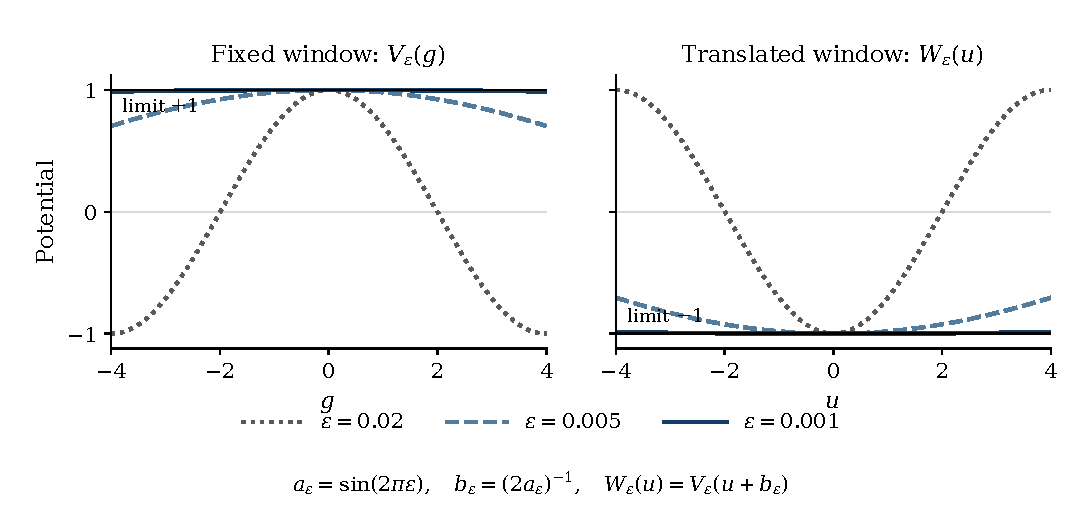
\includegraphics[width=\linewidth]{pictures/dynamical_potential_locality}
\caption{Fixed and translated windows for the shear-torus potentials,
with $V_\varepsilon=V_{z_\varepsilon}$ in the plot.
As $\varepsilon\downarrow0$, $V_{z_\varepsilon}$ tends to $1$ on each
fixed bounded window, while
$W_\varepsilon(u)=V_{z_\varepsilon}(u+b_\varepsilon)$ tends to $-1$,
with $b_\varepsilon\to\infty$. The curves show the explicit potentials,
not numerical approximations to their semigroups.}
\label{fig:dynamic_potential_windows}
\end{figure}

More explicitly, the conjugation identities are
\[
\begin{aligned}
U_{b_\varepsilon}(H_0+V_{z_\varepsilon})U_{b_\varepsilon}^{-1}
 &=H_0+W_\varepsilon,\\
U_{b_\varepsilon}S_{z_\varepsilon}(t)U_{b_\varepsilon}^{-1}
 &=e^{-t(H_0+W_\varepsilon)}.
\end{aligned}
\]
The potentials $W_\varepsilon$ are bounded by one. The same Duhamel
and dominated-convergence argument just proved, now comparing these
potentials directly with the constant $-1$, gives
\[
e^{-t(H_0+W_\varepsilon)}f\longrightarrow e^tP_tf
\qquad(f\in L^2).
\]
The member $S_{z_0}(t)=e^{-t}P_t$ is unchanged by translation.
Unitary invariance of the norm therefore implies, for any unit vector $f$,
\[
\liminf_{\varepsilon\downarrow0}
\|S_{z_\varepsilon}(t)-S_{z_0}(t)\|
\geq(e^t-e^{-t})\|P_tf\|_2.
\]
Here $\|P_t\|_{2\to2}=1$: the upper bound is known, and a unit vector
whose Fourier transform is supported in $\{|\xi|<\delta\}$ gives
$\|P_tf\|_2\geq e^{-t\delta^2}$. Letting $\delta\downarrow0$
proves the desired lower bound.

For the upper bound, the two-sided Gaussian estimates with $M=1$ give
\[
0\leq K_{z_\varepsilon}(t,x,y)-e^{-t}p_t(x-y)
\leq(e^t-e^{-t})p_t(x-y).
\]
Integration against $|f|$ and the $L^2$ contraction property of $P_t$
show that the operator norm of the difference is at most $e^t-e^{-t}$.
This proves \eqref{eq:dynamic_norm_discontinuity}. Nevertheless the
strong-continuity proposition applies, and the earlier weighted
Lipschitz estimate gives convergence of $k_t(z_\varepsilon,\cdot)$
to $k_t(z_0,\cdot)$ in every $C_a$. The loss of operator-norm
continuity comes from spatial translates moving out to infinity,
which are not controlled uniformly by convergence of this single row.

\subsection{Application to spectra over invariant subsystems}
The preceding counterexample concerns operator norm at individual phases.
There is a different useful consequence of the kernel estimates: spectral
continuity when entire invariant subsystems are compared. We give a direct
Euclidean heat-kernel proof of the localization argument in
\textcite[Lemmas~4.2--4.3 and Theorem~4.6]{BeckusTakase2025Spectral}.
Smooth cutoffs, the Gaussian first moment, and the localized operator
estimate supply the needed bounds. Only the self-adjoint spectral
calculus already used in the thesis is imported in this proof.

Let $\mathcal S$ be the collection of nonempty closed subsets of $Z$
invariant under every $T(g,\cdot)$. For $X,Y\in\mathcal S$, write
\[
d_H(X,Y)=\max\left\{
 \sup_{x\in X}\inf_{y\in Y}d_Z(x,y),
 \sup_{y\in Y}\inf_{x\in X}d_Z(x,y)\right\}.
\]
For each fixed $t>0$ define the compact spectral set
\[
\Sigma_t(X)=\overline{\bigcup_{z\in X}\sigma(e^{-tH_z})}
 \subseteq[0,e^{Mt}].
\]
The overline denotes closure in $\mathbb R$. Each spectrum is nonempty,
and operator positivity from spectral calculus and the norm bound for the heat
operator give the displayed inclusion, hence compactness.

\begin{lemma}[Averaged localization of a heat operator]
\label{lem:dynamic_spectral_localization}
Fix a real function $\chi\in C_c^1(B(0,1))$ with $\|\chi\|_2=1$,
and put $G_\chi=\|\nabla\chi\|_2$. For $R>0$ and $a\in\mathbb R^d$,
let $\chi_{a,R}(x)=R^{-d/2}\chi((x-a)/R)$, also denoting the
corresponding multiplication operator. Write $S_z=e^{-tH_z}$ for a
fixed $t>0$, and define
\[
B_t=e^{Mt}\sqrt{2dt}\,G_\chi.
\]
For every $f\in L^2$,
\[
\int\|\chi_{a,R}f\|_2^2\,da=\|f\|_2^2,\qquad
\left(\int\|[S_z,\chi_{a,R}]f\|_2^2\,da\right)^{1/2}
\leq \frac{B_t}{R}\|f\|_2.
\]
\end{lemma}
\Proof
Tonelli and the change of variable $u=(x-a)/R$ give the first identity.
Write $\chi_R=\chi_{0,R}$. The fundamental theorem of calculus
along a segment, followed by the triangle inequality in $L^2$, gives
\[
\|\chi_R(\cdot+r)-\chi_R\|_2
\leq |r|\|\nabla\chi_R\|_2
=\frac{|r|G_\chi}{R}.
\]
The commutator has the absolutely convergent kernel expression
\[
([S_z,\chi_{a,R}]f)(x)
=\int K_z(t,x,x+r)
 [\chi_R(x+r-a)-\chi_R(x-a)]f(x+r)\,dr.
\]
Absolute convergence at each $a,x$ follows from the Gaussian bound,
boundedness of $\chi_R$, and Cauchy--Schwarz against $f$.
All these integrands are jointly measurable. Put
$m_t=\int|r|p_t(r)\,dr\leq\sqrt{2dt}$. Scalar Cauchy--Schwarz,
with weight $|r|p_t(r)$, gives
\[
|([S_z,\chi_{a,R}]f)(x)|^2
\leq e^{2Mt}m_t\int\frac{p_t(r)}{|r|}
 |\chi_R(x+r-a)-\chi_R(x-a)|^2|f(x+r)|^2\,dr.
\]
The value at $r=0$ is irrelevant. This inequality is valid with an
infinite right side; the next calculation proves its integrability.
For each fixed $r$, integration in $a$ of the squared difference equals
$\|\chi_R(\cdot+r)-\chi_R\|_2^2$, independently of $x$.
Tonelli and translation invariance in $x$ therefore give
\[
\begin{split}
\int\|[S_z,\chi_{a,R}]f\|_2^2\,da
&\leq e^{2Mt}m_t\|f\|_2^2
  \int\frac{p_t(r)}{|r|}
  \|\chi_R(\cdot+r)-\chi_R\|_2^2\,dr\\
&\leq\frac{e^{2Mt}m_t^2G_\chi^2}{R^2}\|f\|_2^2
\leq\frac{B_t^2}{R^2}\|f\|_2^2.
\end{split}
\]
This proves the commutator estimate using only scalar
Cauchy--Schwarz and Tonelli.
\Done

\begin{corollary}[Spectral continuity of invariant subsystems]
\label{cor:dynamic_subsystem_spectra}
Under the original Lipschitz sampling and linear action-growth
hypotheses, fix the normalized cutoff from
Lemma~\ref{lem:dynamic_spectral_localization} and put
\[
Q_t=LCe^{Mt},\qquad b_d=c_d+\sqrt{d/2},\qquad
A_t=\max\{e^{Mt},\ B_t+Q_t(2t+b_dt^{3/2})\}.
\]
For all nonempty closed invariant subsets $X,Y$ of $Z$,
\[
\operatorname{dist}_H(\Sigma_t(X),\Sigma_t(Y))
\leq A_t d_H(X,Y)^{1/2}.
\]
\end{corollary}
\Proof
Let $\delta=d_H(X,Y)$. If $\delta=0$, compactness and closedness give
$X=Y$, and the claim is immediate. First suppose $0<\delta\leq1$.
Fix $z\in X$ and $\lambda\in\sigma(S_z)$. Since $S_z$ is bounded
self-adjoint, for every $\epsilon>0$ there is a unit vector $f$ with
$\|(S_z-\lambda)f\|_2<\epsilon$. To see this from the spectral theorem,
its spectral projection on $(\lambda-\epsilon,\lambda+\epsilon)$ is
nonzero; otherwise the spectral integral of $(s-\lambda)^{-1}$ would
supply a bounded inverse to $S_z-\lambda$. Normalize a nonzero vector
in that projection's range.

For any $R>0$, use
\[
(S_z-\lambda)\chi_{a,R}f
=\chi_{a,R}(S_z-\lambda)f+[S_z,\chi_{a,R}]f.
\]
The localization lemma and the triangle inequality in $L^2(da;L^2)$
give
\[
\left(\int\|(S_z-\lambda)\chi_{a,R}f\|_2^2\,da\right)^{1/2}
\leq\epsilon+B_t/R,
\qquad \int\|\chi_{a,R}f\|_2^2\,da=1.
\]
These are measurable functions of $a$; for example,
$a\mapsto\chi_{a,R}f$ is norm continuous, since translates of the
compactly supported continuous function $\chi_R$ vary continuously in
supremum norm. For every $\eta>0$, there is therefore an $a$ with
$\chi_{a,R}f\ne0$ and
\[
\frac{\|(S_z-\lambda)\chi_{a,R}f\|_2}{\|\chi_{a,R}f\|_2}
\leq\epsilon+B_t/R+\eta.
\]
Otherwise the squared numerator would be at least
$(\epsilon+B_t/R+\eta)^2$ times the squared denominator almost
everywhere, contradicting the two integral bounds.

Normalize this localized vector and translate it with
$(U_au)(x)=u(x+a)$. The resulting unit vector $v$ is supported in
$B(0,R)$. Translation of the potential gives
\[
U_aS_zU_a^{-1}=S_{T(a,z)}.
\]
Thus $z'=T(a,z)\in X$ and
$\|(S_{z'}-\lambda)v\|_2\leq\epsilon+B_t/R+\eta$.
Compactness of $Y$ supplies $w\in Y$ with $d_Z(z',w)\leq\delta$.
Proposition~\ref{prop:dynamic_local_operator_lipschitz}, applied to the
ball of radius $R$, yields
\[
\|(S_{z'}-S_w)v\|_2
\leq Q_t\,[t(1+R)+b_dt^{3/2}]\delta.
\]
Spectral calculus for the self-adjoint operator $S_w$ gives
$\operatorname{dist}(\lambda,\sigma(S_w))
\leq\|(S_w-\lambda)v\|_2$. Consequently
\[
\operatorname{dist}(\lambda,\Sigma_t(Y))
\leq\epsilon+\eta+B_t/R
 +Q_t[t(1+R)+b_dt^{3/2}]\delta.
\]
Let $\epsilon,\eta$ decrease to zero; the resulting bound is independent
of the chosen localizations and of $w$. Choose $R=\delta^{-1/2}$ and
use $\delta\leq\sqrt\delta$ to bound the right side by
\[
[B_t+Q_t(2t+b_dt^{3/2})]\sqrt\delta.
\]
The bound is uniform in $z\in X$ and $\lambda\in\sigma(S_z)$.
Distance to the closed set $\Sigma_t(Y)$ is continuous, so it extends
to every $\lambda\in\Sigma_t(X)$. Interchanging $X,Y$ gives the other
directed distance, proving the desired Hausdorff bound for
$0<\delta\leq1$.

Finally, if $\delta>1$, both nonempty spectral sets lie in $[0,e^{Mt}]$.
Their Hausdorff distance is at most $e^{Mt}\leq e^{Mt}\sqrt\delta$.
The stated maximum therefore works for every $\delta$.
\Done

\begin{corollary}[Qualitative spectral continuity under continuous sampling]
\label{cor:dynamic_subsystem_spectra_continuous}
Suppose only that $Z$ is a nonempty compact metric space, $T$ is a
continuous action of $\mathbb R^d$ on $Z$, and $v:Z\to\mathbb R$ is
continuous. For each fixed $t>0$, the map
$X\mapsto\Sigma_t(X)$ on nonempty closed invariant subsets of $Z$
is uniformly continuous for Hausdorff distance.
\end{corollary}
\Proof
Put $M=\|v\|_\infty$, and retain the cutoff and constant $B_t$ from
Lemma~\ref{lem:dynamic_spectral_localization}. That lemma uses only the
uniform Gaussian bound, so it remains valid under the present
hypotheses. For $R>0$, let $\chi_{B_R}$ be multiplication by the
indicator of $B(0,R)$, and define
\[
\omega_R(\delta)=\sup_{\substack{z,w\in Z\\d_Z(z,w)\leq\delta}}
 \|(S_z(t)-S_w(t))\chi_{B_R}\|_{2\to2},\qquad \delta\geq0.
\]
Proposition~\ref{prop:dynamic_strong_parameter_continuity} gives
operator-norm continuity of $z\mapsto S_z(t)\chi_{B_R}$.
Compactness of $Z$ makes this map uniformly continuous, and hence
$\omega_R(\delta)\to0$ as $\delta\downarrow0$ for each fixed $R$.

The localization and recentering argument in the proof of
Corollary~\ref{cor:dynamic_subsystem_spectra} uses the quantitative
hypotheses only when comparing the two operators on a vector supported
in $B(0,R)$. Replacing that comparison by the definition of
$\omega_R$ gives, for every $R>0$,
\[
\operatorname{dist}_H(\Sigma_t(X),\Sigma_t(Y))
 \leq \frac{B_t}{R}+\omega_R(d_H(X,Y)).
\]
Indeed, a localized approximate spectral vector for a phase in $X$
can be translated into $B(0,R)$; invariance keeps its translated phase
in $X$, and compactness of $Y$ supplies a phase within $d_H(X,Y)$.
The displayed modulus bounds the operator difference on that vector.
Letting the approximate-vector errors vanish, passing to spectral
closures, and interchanging $X,Y$ proves the inequality.
Given a positive error tolerance, first choose $R$ large and then
choose $d_H(X,Y)$ small. Both choices are independent of $X,Y$,
which proves uniform continuity.
\Done

\paragraph{Comparison with the general group theorem.}
The quantitative proof uses the original metric and linear action bound.
The following normalization additionally explains how the setting fits
\textcite[Theorem~1.3(a)]{BeckusTakase2025Spectral}, whose action bound
has coefficient one at the group identity.

\begin{lemma}[An adapted metric for the action]
\label{lem:dynamic_adapted_metric}
Under the original linear-growth hypothesis, put $C_0=\max\{1,C\}$ and
\[
d_*(z,w)=\sup_{g\in\mathbb R^d}
 \frac{d_Z(T(g,z),T(g,w))}{1+|g|}.
\]
Then $d_*$ is a metric with the same compact topology as $d_Z$, and
\[
d_Z\leq d_*\leq C_0d_Z,\qquad
 d_*(T(h,z),T(h,w))\leq(1+|h|)d_*(z,w).
\]
The sampling function $v$ remains Lipschitz with constant at most $L$.
\end{lemma}
\Proof
The assumed growth bound makes the supremum finite. Symmetry and the
triangle inequality follow from those of $d_Z$, taking suprema; the
term $g=0$ gives $d_*(z,w)\geq d_Z(z,w)$ and hence definiteness.
The two metric inequalities imply equivalence of their topologies and
preserve compactness. With $u=g+h$, the triangle inequality in
$\mathbb R^d$ gives
\[
1+|u|\leq(1+|u-h|)(1+|h|).
\]
Reindexing the supremum proves the action estimate. The sampling bound is
\[
|v(z)-v(w)|\leq Ld_Z(z,w)\leq Ld_*(z,w).
\]
\Done

Let $d_{H,*}$ denote Hausdorff distance induced by $d_*$.
The metric comparison gives $d_H\leq d_{H,*}\leq C_0d_H$ on
nonempty closed subsystems. With $\tau(g,z)=T(-g,z)$ and
$\kappa_t(r,z)=k_t(z,r)$, the operator convention in that theorem is
\[
(A_zf)(g)=\int\kappa_t(h-g,\tau(-g,z))f(h)\,dh
        =e^{-tH_z}f(g).
\]
The adapted action has bound $1+|g|$. Applying
Theorem~\ref{thm:dynamic_kernel_lipschitz} in $d_*$ gives an integrable
parameter-Lipschitz envelope, since it is a Gaussian times a linear
polynomial in $|r|$. The Gaussian bound also gives uniform integrability
and a uniform first moment, including suprema along translated orbits.
The heat operators are self-adjoint and hence normal. Finally,
$\mathbb R^d$ with its proper translation-invariant Euclidean metric
is unimodular and has ball volume $\omega_d r^d$, so the group's required
two-sided volume-growth condition holds. Thus the general theorem gives
another route to the result; its kernel hypotheses are verified rather
than assumed for the Schr\"odinger family.

\begin{corollary}[The bottom of the subsystem spectrum]
Under the baseline quantitative hypotheses, for $X\in\mathcal S$ let
\[
E(X)=\inf\bigcup_{z\in X}\sigma(H_z).
\]
Then $-M\leq E(X)\leq M$, and for every $t>0$,
\[
|E(X)-E(Y)|\leq\frac{e^{tM}}{t}A_t d_H(X,Y)^{1/2}.
\]
This statement concerns a spectral infimum; it does not assert that
there is an eigenvector at that energy.
\end{corollary}
\Proof
The operator inequality $H_z\geq-M$ proves the lower bound.
For any $\delta>0$, choose a unit vector whose Fourier transform is
supported in $\{|\xi|^2<\delta\}$. It belongs to $D(H_0)=D(H_z)$
and satisfies
\[
\langle H_zf,f\rangle
 =\int |\xi|^2|\widehat f(\xi)|^2\,d\xi
   +\int V_z(x)|f(x)|^2\,dx\leq\delta+M.
\]
Spectral calculus gives $\inf\sigma(H_z)\leq\langle H_zf,f\rangle$.
Letting $\delta\downarrow0$ proves the upper bound for each phase,
and hence for the nonempty subsystem.
Spectral mapping and the definition of infimum give
\[
\max\Sigma_t(X)=e^{-tE(X)}\in[e^{-tM},e^{tM}].
\]
Maxima of nonempty compact real sets differ by at most their Hausdorff
distance. On this interval the derivative of $-(1/t)\log s$ has
absolute value at most $e^{tM}/t$. Applying this Lipschitz bound to the
two maxima and then Corollary~\ref{cor:dynamic_subsystem_spectra}
proves the estimate.
\Done

The objects compared here are invariant subsystems, not arbitrary pairs
of individual phases. Moreover the spectral sets belong to the bounded
heat operators. By spectral mapping,
\[
\sigma(e^{-tH_z})=\overline{\{e^{-tE}:E\in\sigma(H_z)\}}.
\]
Passing back to unbounded energies uses a logarithm whose derivative
is unbounded near zero. No unweighted Hausdorff estimate for the
unbounded Schr\"odinger spectra, or for their intersections with a
sharp energy window, is asserted. The direct Euclidean argument specializes the cited localization
method; no new general spectral-continuity principle is claimed.

\begin{example}[The shear family and its limiting subsystem]
For the shear-torus family above, fix $t>0$ and define
\[
X_\varepsilon=\{[\varepsilon,y]:y\in\mathbb R/\mathbb Z\},\qquad
X_0=\{[0,y]:y\in\mathbb R/\mathbb Z\}.
\]
For $0<\varepsilon<1/4$, the nonzero speed
$a_\varepsilon=\sin(2\pi\varepsilon)$ makes the orbit of
$z_\varepsilon$ equal to $X_\varepsilon$: as $g$ ranges over
$\mathbb R$, $ga_\varepsilon$ ranges over $\mathbb R$.
The quotient Euclidean metric gives
$d_H(X_\varepsilon,X_0)=\varepsilon$, by matching second coordinates
and minimizing the first-coordinate distance. But the orbit of $z_0$
is only the singleton $\{z_0\}$, not $X_0$.

All phases in $X_\varepsilon$ give unitarily equivalent operators:
translation by $b$ conjugates $H_z$ to $H_{T(b,z)}$, and the action
is transitive on this circle. Thus
$\Sigma_t(X_\varepsilon)=\sigma(S_{z_\varepsilon}(t))$.
On $X_0$ each potential is the constant $\cos(2\pi y)$.
The Fourier multiplier $|\xi|^2$ has essential range $[0,\infty)$,
so $\sigma(H_0)=[0,\infty)$. Spectral mapping therefore gives
\[
\sigma(e^{-t(H_0+c)})=[0,e^{-tc}]\quad(c\in\mathbb R),
\qquad \Sigma_t(X_0)=[0,e^t].
\]
Corollary~\ref{cor:dynamic_subsystem_spectra} now proves
\[
\operatorname{dist}_H\bigl(\sigma(S_{z_\varepsilon}(t)),[0,e^t]\bigr)
 \leq A_t\sqrt{\varepsilon}.
\]
In contrast, $\sigma(S_{z_0}(t))=[0,e^{-t}]$. The triangle inequality
for Hausdorff distance, applied with this fixed interval, yields
\[
\lim_{\varepsilon\downarrow0}
\operatorname{dist}_H\bigl(\sigma(S_{z_\varepsilon}(t)),
                         \sigma(S_{z_0}(t))\bigr)=e^t-e^{-t}.
\]
Thus even the phase spectra are discontinuous here. The subsystem
spectra converge to the spectrum of the limiting circle, which is
larger than the orbit of the limiting phase. This conclusion follows from the spectral localization argument;
the earlier operator-norm limit has its separate direct proof.
\end{example}

\ifdefined\qwertyflag
\undef\qwertyflag
\end{document}
\fi

